\documentclass[14pt]{beamer}
\usepackage{graphicx}
\usepackage{fontspec}
\setsansfont{Minion Pro}


\usetheme{UofA}
\newcommand*\chem[1]{\ensuremath{\footnotesize{\mathrm{#1}}}}
\newcommand*\figcite[1]{\vspace*{\fill}\raggedleft\footnotesize{#1}}

\title[Condensate Cloud]{Condensate Clouds of \\Cool Objects}
\author{Yifan Zhou}
\institute[UofA]{Stewart Observatory\\
University of Arizona}
\begin{document}

{\setbeamertemplate{footline}{}
  \setbeamertemplate{background canvas}[vertical
  shading][bottom=UA_BLUE!15,top=white!20]
  \setbeamertemplate{background}{  \vbox to \paperheight{\vfil\hbox to
      \paperwidth{\hfil
\includegraphics[width=1.5in]{ua_triangle_blue_low}\hfil}}%
    }

\begin{frame}
\maketitle
\end{frame}}

\begin{frame}
  \frametitle{Clouds}
  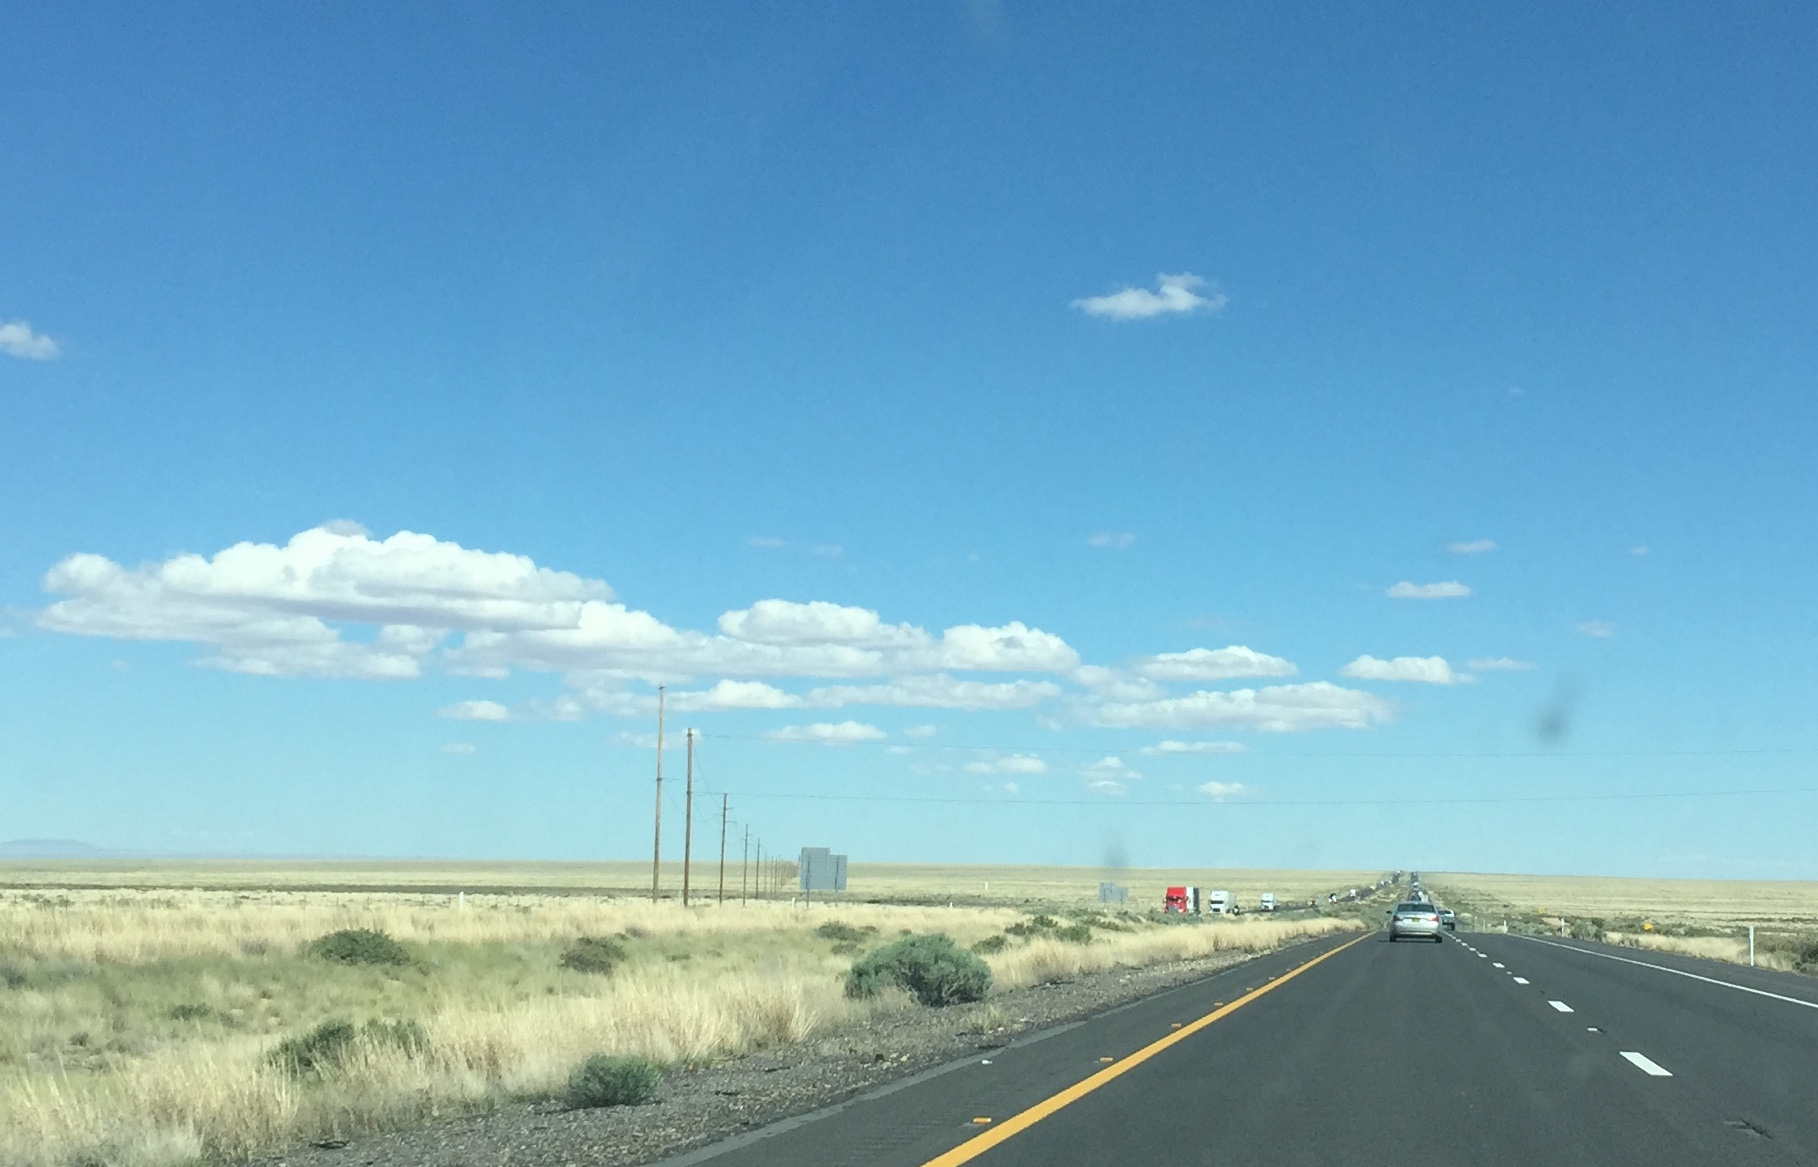
\includegraphics[width=\textwidth]{cloudsonearth}\\
  \figcite{on the way to meteor crater}
\end{frame}

\begin{frame}
  \frametitle{Uniqueness of Low T Atmosphere}
\begin{itemize}
\item Complex chemistry and molecules
\item Alkali opacity
\item \textbf{{Condensation and cloud formation}\\
 Condensate species:\\
 \chem{MgSi_{3}},  \chem{Mg_{2}Si_{4}}, ...\\
to \chem{H_{2}O}, \chem{NH_{3}},...}
\end{itemize}
\end{frame}

\begin{frame}
  \frametitle{Cloud Keynotes}
  \only<1>{  \structure{What does cloud mean?}
    \begin{itemize}
    \item solid/liquid particles formed by condensation
    \end{itemize}
}
\only<2-3>{
    \only<2>{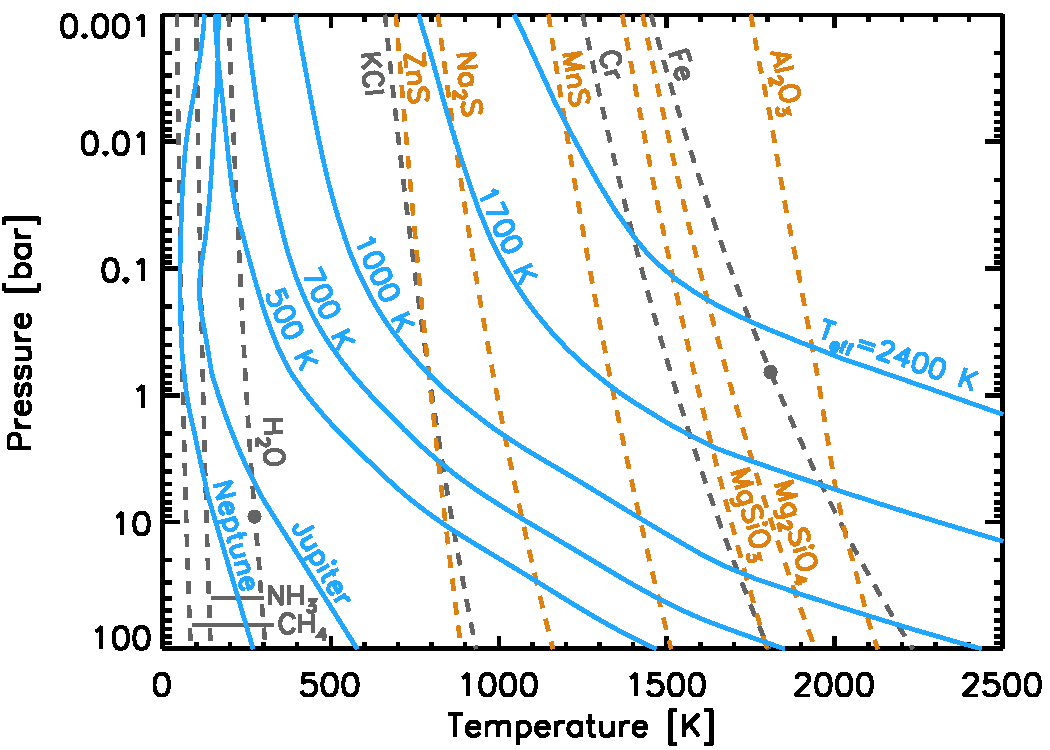
\includegraphics[height= 0.8\textheight]{cond_curves_Fig9}\\
    \figcite{Marley \& Robinson 2014}}
  \only<3>{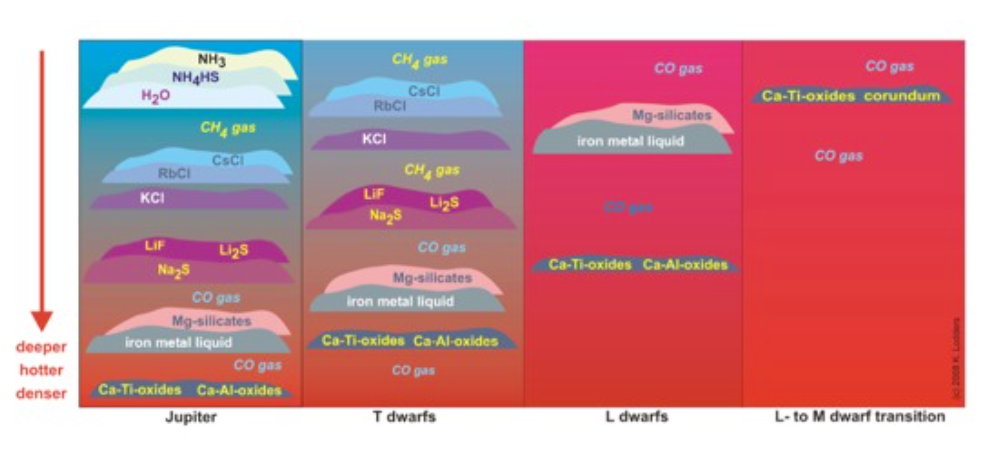
\includegraphics[width=\textwidth]{cloudsonothers}}
}

\only<4>{\structure{Physical processes}
    \begin{itemize}
  \item dust particle formation
  \item the mixing of dust and gas
  \item dust growth and evaporation
  \item the feedback of condensation to chemical equilibrium.
  \end{itemize}}
% \only<5>{\structure{Cloud Opacity}
% { \footnotesize \[
%     \tau_\lambda = 75 \epsilon Q^{\rm ext}_{\lambda}(r_{\rm c}) \varphi \biggl({P_{\rm c}\over {1~\rm bar}}\biggr) \biggl({{10^5~\rm cm\,s^{-2}}\over g}\biggr)\biggl({{1~\rm \mu m}\over r_{\rm c}}\biggr)\biggl({{1~\rm g\,cm^{-3}}\over \rho_{\rm c}}\biggr) \
%   \]}
% {\normalsize $r_{\rm c}$ -- particle size\\
% $Q^{\rm ext}_{\lambda}(r_{\rm c})$ -- extinction efficiency\\}
% \figcite{Marley \& Robinson (2014)}}
\only<6>{\structure{Lack of constraints}
  \begin{itemize}
    \item degeneracy of spectroscopy
  \end{itemize}
}
\end{frame}
% \begin{frame}
%   \frametitle{Spectrum}
%   
% \end{frame}

\begin{frame}
  \frametitle{Model Approaches}
  \only<1>{
    \structure{Tsuji Model}
    \begin{itemize}
    \item Precipitation described by critical temperature
      $T_{\mathrm{cr}}$
      \item Cloud thickness varies with  $T_{\mathrm{cr}}$
    \end{itemize}
  }
  \only<2>{
    \structure{Allard settl model}
    \begin{itemize}
    \item mixing, condensate, coagulation, and sedimentation time
      scales are bonded by particle size and condensate fraction
    \item particle size and condensate fraction are calculated to
      balance those time scales
    \end{itemize}
  }
  \only<3>{
    \structure{Ackerman \& Marley}
    \begin{itemize}
    \item using a scaling factor to describe the relationship of
      sedimentation velocity and turbulent mixing
    \item prescribing a particle size distribution 
    \end{itemize}
  }
  \only<4>{
    \structure{Helling \& Woitke}
    \begin{itemize}
    \item Condensation starts with formation of seed particles
    \item seeds growing by gas-solid surface reaction
    \end{itemize}
  }
  % \begin{tabular}{llll}
  %   Model&\textit{Settl}&A\&M&H\&W \\\hline
  %        condensation&fixed ss& remove condensate from gas&dust formed
  %                                                           on
  %                                                           nucleation \\
  %        vertical mixing&$\tau_{\mathrm{mix}}$&$f_{\mathrm{sed}}$&
  % \end{tabular}
  % A\&M: Ackerman\&Marley, H\&W: Helling\&Woitke\\
  % ss: supersaturation
\end{frame}

\begin{frame}
  \frametitle{Comparison}
  \begin{columnsonlytextwidth}
    \begin{column}{0.35\textwidth}
      \centering
      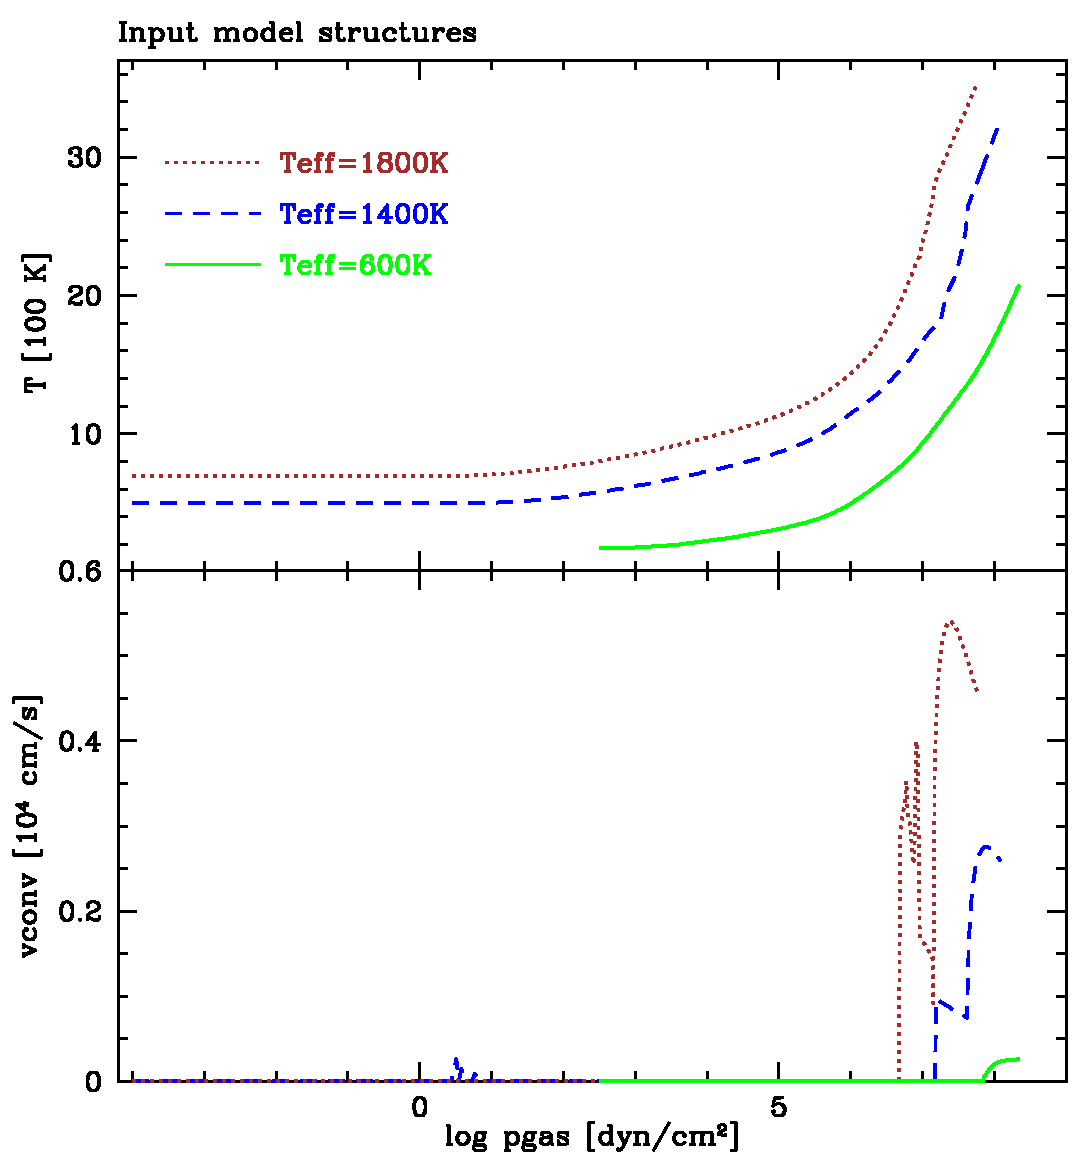
\includegraphics[width=\columnwidth]{InputStructure}
    \end{column}
    \begin{column}{0.6\textwidth}
      \centering
      \only<1>{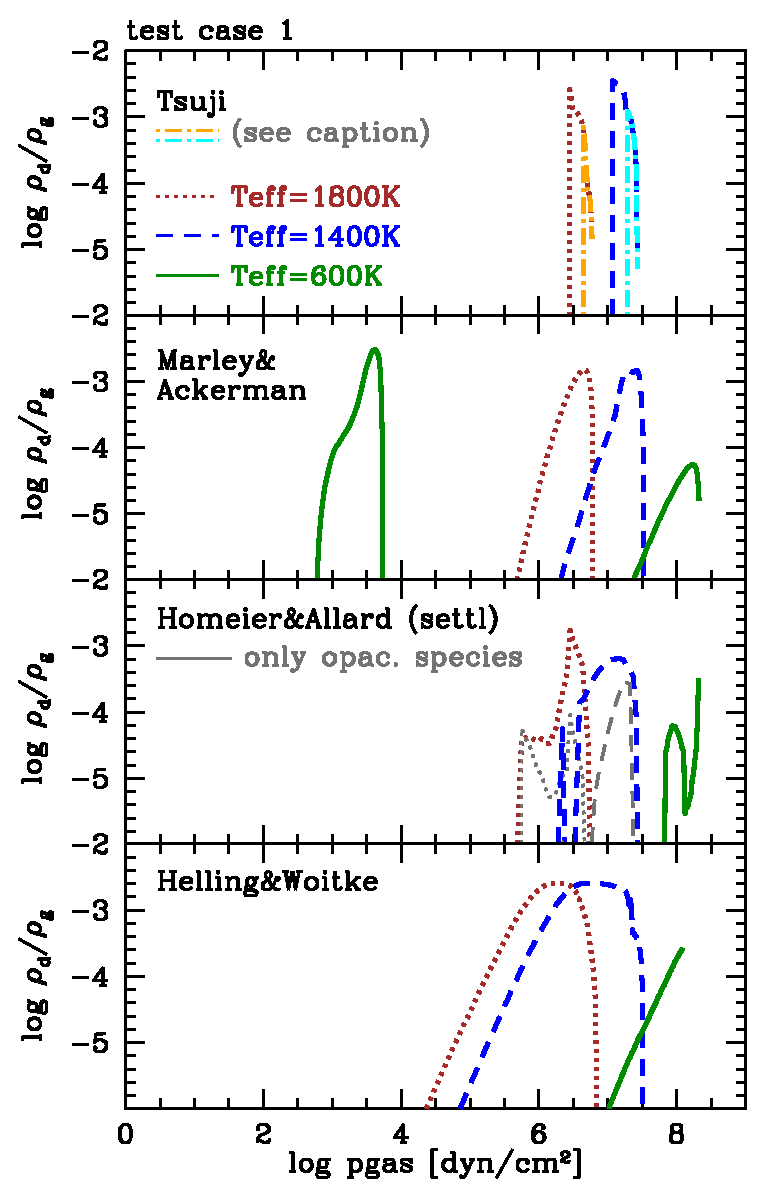
\includegraphics[height=0.8\textheight]{RhodRhoG}}
      \only<2>{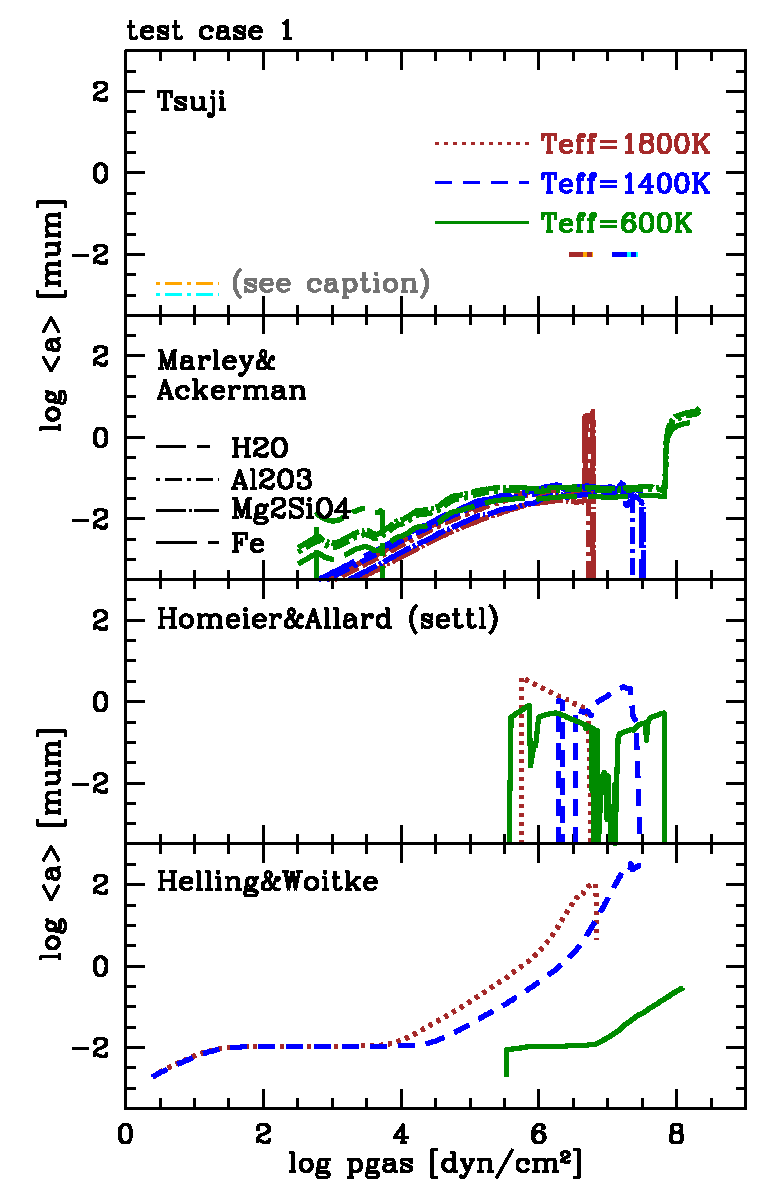
\includegraphics[height=0.8\textheight]{AmeanTC1}}
    \end{column}
  \end{columnsonlytextwidth}
  \figcite{Helling et. al. (2008)}
\end{frame}

\begin{frame}
  \frametitle{Comparison}
  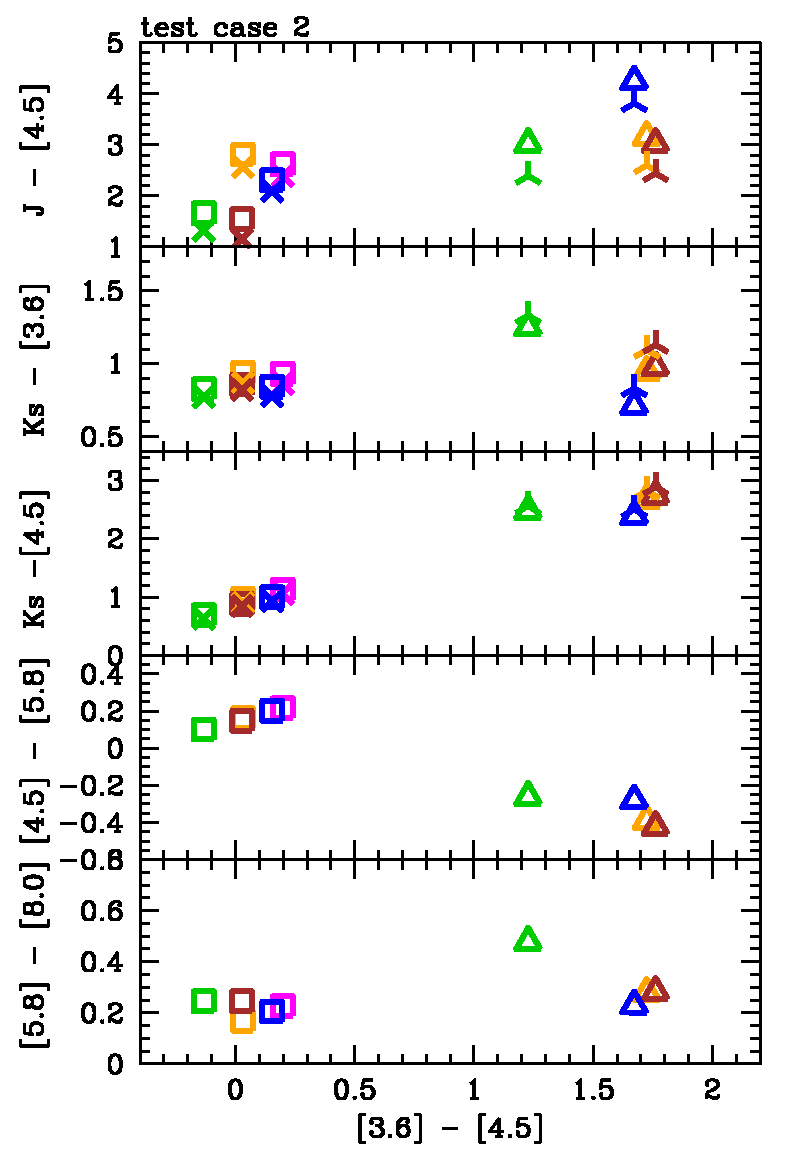
\includegraphics[width=\columnwidth]{Colours}
\end{frame}


% \begin{frame}
%   \frametitle{Patchy Cloud}
%   \begin{itemize}
%   \item Variability of brown dwarfs
%   \item under-luminosity of direct imaged exoplanets and brown dwarfs.
%   \end{itemize}
% \end{frame}

\begin{frame}
  \frametitle{Time resolved observation}
  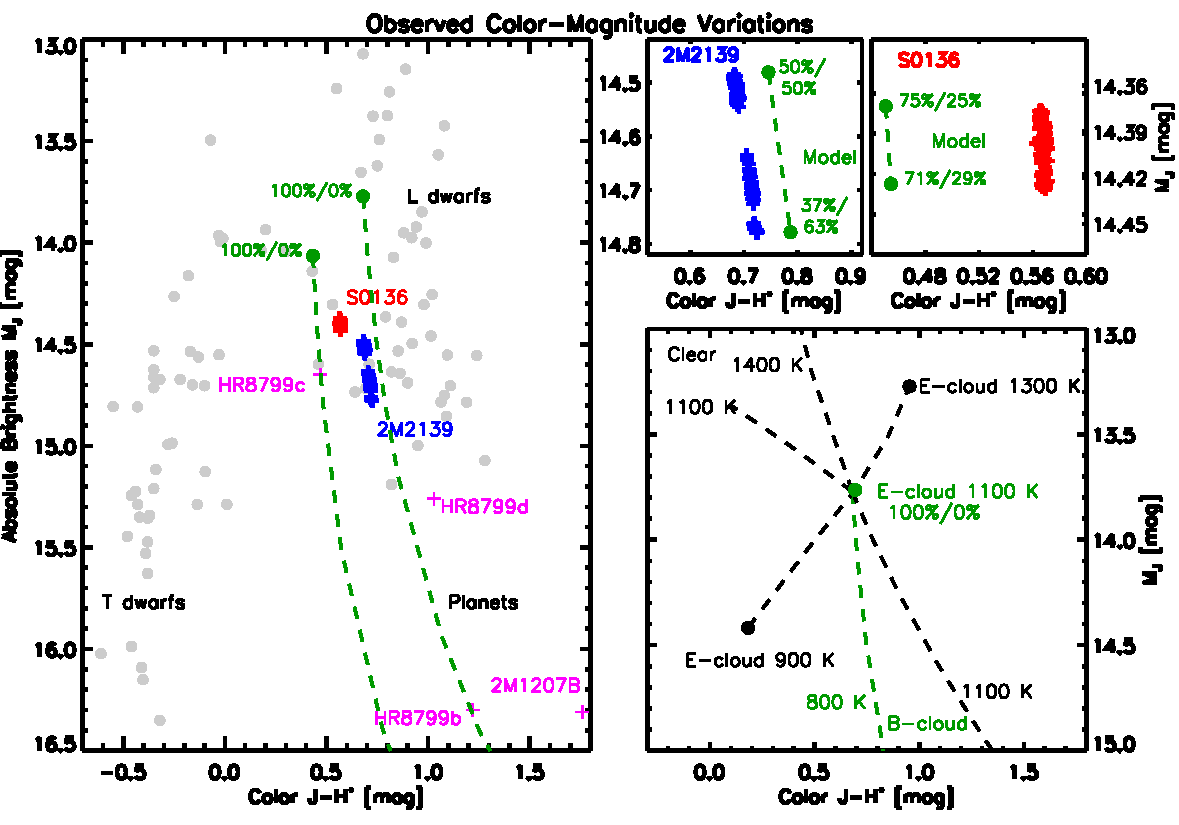
\includegraphics[width=\textwidth]{CMD}\\
  \figcite{Apai et. al. (2013)}
\end{frame}

\begin{frame}
  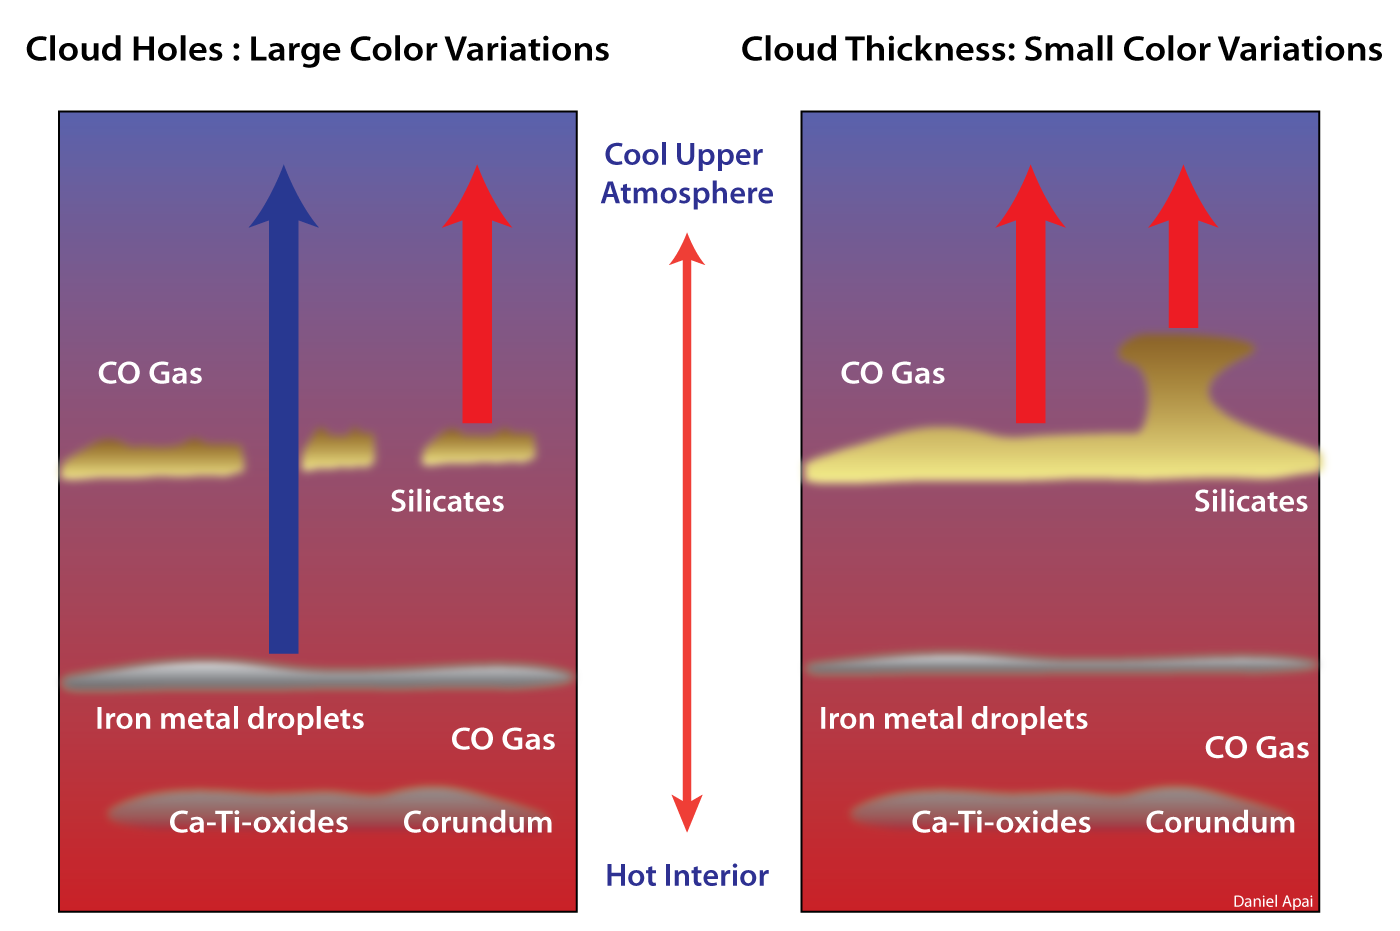
\includegraphics[height=0.8\textheight]{varyThick}
\end{frame}



\end{document}


%%% Local Variables:
%%% mode: latex
%%% TeX-master: t
%%% End:
